\documentclass[11pt]{article}
\usepackage[a4paper,margin=2.6cm]{geometry}
\usepackage[T1]{fontenc}
\usepackage{lmodern}
\usepackage{microtype}
\usepackage{amsmath,amssymb,amsthm,mathtools}
\usepackage{booktabs}
\usepackage{graphicx}
\usepackage{enumitem}
\usepackage{xcolor}
\usepackage[colorlinks=true,linkcolor=blue!50!black,citecolor=blue!50!black,urlcolor=blue!50!black]{hyperref}

\theoremstyle{plain}
\newtheorem{theorem}{Theorem}
\newtheorem{lemma}[theorem]{Lemma}
\newtheorem{proposition}[theorem]{Proposition}
\newtheorem{corollary}[theorem]{Corollary}
\theoremstyle{definition}
\newtheorem{definition}[theorem]{Definition}
\theoremstyle{remark}
\newtheorem{remark}[theorem]{Remark}

\newcommand{\cw}{\mathrm{cw}}
\newcommand{\ccw}{\mathrm{ccw}}

\title{The $9/8$ lower bound for ring loading:\\ an independent rediscovery with exact proofs}
\author{Thanh Van Nguyen\\[2pt]
\small Tsinghua Shenzhen International Graduate School, Tsinghua University, Shenzhen, China\\
\small \texttt{felicenguyen2001@gmail.com}}
\date{November 2026}

\begin{document}
\maketitle

\begin{abstract}
In the ring loading problem, demands between pairs of nodes of a cycle must each be routed, unsplit, clockwise or counterclockwise so that the maximum edge load~$L$ is as small as possible.
Schrijver, Seymour and Winkler (1998) proved $L \le L^* + \tfrac32 D$, where $L^*$ is the optimum when demands may be split and $D$ is the largest demand.
The best constant is open. Skutella (2016) gave an instance with $L = L^* + \tfrac{11}{10}D$, and Däubel (2022) proved $L \le L^* + \tfrac{13}{10}D$.
We give a ring with 43 nodes and 55 demands, at most one demand per pair of nodes, for which $L = L^* + \tfrac98 D$. So the constant is at least $9/8$.
The instance is built from a 15-term sequence that also gives the value $9/8$ for the closely related sequence constant of Schrijver, Seymour and Winkler. That constant is Problem~6.61 in the AlphaEvolve problem list of Georgiev, Gómez-Serrano, Tao and Wagner.
All data are multiples of $1/16$, and both bounds have exact, computer-checked proofs that run in seconds.
\emph{Priority:} neither bound is new. The value $9/8$ for the sequence constant was posted first by the GitHub user Maks23 on 8 October 2026, and Lemma~7 of Däubel (2022) turns such a sequence into a ring with gap $\tfrac98 D$. We found our instance independently; this note records it as an independent rediscovery with a second set of exact proofs.
\end{abstract}

\section{Introduction}

\paragraph{The problem.}
Let $C_n$ be the cycle with nodes $0,\dots,n-1$ and edges $e=\{e,e+1\}$, where node and edge indices are taken modulo~$n$.
A ring loading instance is a list of demands $d_j\ge 0$ between node pairs $\{s_j,t_j\}$.
An \emph{unsplittable routing} sends each demand entirely clockwise or entirely counterclockwise.
A \emph{split routing} may send any fraction of a demand clockwise and the rest counterclockwise.
The load of an edge is the total amount routed through it.
Let $L$ and $L^*$ be the smallest possible maximum edge load over unsplittable and split routings, respectively, and let $D=\max_j d_j$.
The problem comes from the design of bidirectional SONET rings \cite{CS94}.
Define $\rho$ as the infimum of the constants $c$ such that $L\le L^*+cD$ holds for every instance.

\paragraph{Known bounds.}
Schrijver, Seymour and Winkler \cite{SSW98} proved $\rho\le 3/2$ and gave an instance with $L=L^*+\tfrac{101}{100}D$.
Skutella \cite{Sku16} improved both bounds to $11/10\le\rho\le 19/14$ and disproved a long-standing conjecture of \cite{SSW98}.
Däubel \cite{Dau22} improved the upper bound to $\rho\le 13/10$.
In the published literature, the lower bound $11/10$ had not moved since 2016.
It is still the value quoted in recent work \cite{AS26}.
That paper studies the generalisation to outerplanar supply graphs and proves a lower bound of $4/3$ for that larger class.

Schrijver, Seymour and Winkler related the ring problem to a sequence problem, which we recall in Section~\ref{sec:seq}. For its constant~$\beta$, the bounds $101/100\le\beta\le3/2$ \cite{SSW98} and $11/10\le\beta\le19/14$ \cite{Sku16} are as summarised in \cite{GGTW25}.
The constant $\beta$ is Problem~6.61 in the list of 67 problems studied with AlphaEvolve by Georgiev, Gómez-Serrano, Tao and Wagner \cite{GGTW25}.
There, AlphaEvolve found a sequence of length~15 with value at least $1.119$, improving the bound $11/10$ of \cite{Sku16}.
The public problem repository records this bound as $47/42\approx1.1190$, and still listed it as the record when we wrote this note \cite{AERepo}.
In November 2026 we searched Semantic Scholar and arXiv for work citing \cite{SSW98,Sku16,Dau22,GGTW25}. We found no lower bound above $11/10$ for~$\rho$, and none above $47/42$ for~$\beta$.
That search did not cover the issue tracker of \cite{AERepo}, where both bounds had already appeared.

\paragraph{Priority.}
After the first version of this note we learned of that discussion. Exact certificates for $\beta\ge47/42$ (V.~Yadav, 6 October 2026 \cite{Yad26}) and for $\beta\ge9/8$ (Maks23, 8 October 2026, a sequence of length~14 with entries in $\tfrac1{16}\mathbb{Z}$ \cite{Mak26}) were posted there before our work.
In the same thread, K.~Däubel gave a $9/8$ sequence of length~12 and pointed out that \cite[Lemma~7]{Dau22} turns such a sequence into a ring loading instance with $L-L^*\ge\tfrac98 D$. So $\rho\ge9/8$ also predates this note. The user rozetyp later checked the resulting rings directly with an exact solver \cite{Roz26}.
We have rechecked the certificates of \cite{Mak26} in exact arithmetic.
Our sequence (Table~\ref{tab:seq}) and our ring construction were found independently. The results below are therefore an independent rediscovery with a second set of exact proofs, not new bounds.

\paragraph{Contributions.}
\begin{enumerate}[label=(\arabic*),leftmargin=*]
\item A sequence of length $15$ with entries in $\tfrac1{16}\mathbb{Z}$ that forces the value $9/8$ (Theorem~\ref{thm:seq}). Hence $\beta\ge 9/8$, first shown in \cite{Mak26}.
\item A ring loading instance with $D=1$, $L^*=15/2$ and $L=69/8$ (Theorem~\ref{thm:ring} and Corollary~\ref{cor:distinct}). It has $43$ nodes and $55$ demands on distinct node pairs, or $30$ nodes if a node pair may carry several demands. Hence $\rho\ge 9/8$, which also follows from \cite{Mak26} and \cite[Lemma~7]{Dau22}.
\item Both proofs are exact finite computations. The ring proof reduces to a subset-sum check on $8$ of the $2^{15}$ routings of the long demands (Lemma~\ref{lem:filler}). We release two implementations of this argument, each running in seconds, and a third program that checks the bound by a different argument.
\item Our lift loses part of the gap on AlphaEvolve's sequence (Proposition~\ref{prop:ae}): at most $1.0823\,D$ for the published data, and exactly $\tfrac{23}{21}D$ for a version polished to attain $47/42$ exactly. The construction of \cite[Lemma~7]{Dau22} does not lose it \cite{Roz26}, so this is a limitation of our construction only.
\item We describe the search that found the instance (Section~\ref{sec:search}). We also report that extensive further search stalled at exactly $9/8$.
\end{enumerate}

\section{The sequence constant}\label{sec:seq}

\begin{definition}
Let $m\ge1$ and $u,v\in\mathbb{R}^m_{\ge0}$ with $u_i+v_i\le1$ for all~$i$.
For a sign vector $z\in Z(u,v):=\prod_{i=1}^m\{v_i,-u_i\}$, write
\[
\Delta_k(z)=\sum_{i\le k}z_i-\sum_{i>k}z_i\qquad(0\le k\le m).
\]
For $K\subseteq\{0,\dots,m\}$ let $\alpha_K(u,v)=\min_{z\in Z(u,v)}\max_{k\in K}|\Delta_k(z)|$, and write $\alpha(u,v)=\alpha_{\{1,\dots,m-1\}}(u,v)$, as in the scoring code of \cite{GGTW25,AERepo}.
The constant $\beta$ of \cite{SSW98} is the supremum of $\alpha(u,v)$ over all $m$, $u$ and~$v$.
\end{definition}

Some formulations also include the end terms $k=0$ and $k=m$, both of which equal $|\sum_iz_i|$.
This does not change~$\beta$. Padding $(u,v)$ with one term $u_i=v_i=0$ at each end turns $\alpha_{\{0,\dots,m\}}$ of the old sequence into $\alpha$ of the new one.
Since $\alpha_K$ is monotone in~$K$, a lower bound on $\alpha$ is a lower bound on $\alpha_K$ for every $K\supseteq\{1,\dots,m-1\}$.

\begin{theorem}\label{thm:seq}
For the vectors $u,v$ of Table~\ref{tab:seq} ($m=15$), $\alpha_K(u,v)=9/8$ for every $K$ with $\{1,\dots,14\}\subseteq K\subseteq\{0,\dots,15\}$.
Consequently $\beta\ge 9/8$.
\end{theorem}

\begin{table}[t]
\centering
\caption{The 15-term sequence. The sign vector $z$ attains $\max_k|\Delta_k(z)|=9/8$; the last column lists $\Delta_k(z)$. The end terms are $|\Delta_0(z)|=|\Delta_{15}(z)|=|\sum_iz_i|=9/8$.}\label{tab:seq}
\smallskip
\renewcommand{\arraystretch}{1.15}
\begin{tabular}{rcccr}
\toprule
$k$ & $u_k$ & $v_k$ & $z_k$ & $\Delta_k(z)$\\
\midrule
1 & $\tfrac{3}{4}$ & $\tfrac{1}{8}$ & $-\tfrac{3}{4}$ & $-\tfrac{3}{8}$ \\
2 & $\tfrac{5}{16}$ & $\tfrac{11}{16}$ & $-\tfrac{5}{16}$ & $-1$ \\
3 & $\tfrac{1}{4}$ & $\tfrac{1}{4}$ & $\tfrac{1}{4}$ & $-\tfrac{1}{2}$ \\
4 & $\tfrac{11}{16}$ & $\tfrac{5}{16}$ & $\tfrac{5}{16}$ & $\tfrac{1}{8}$ \\
5 & $\tfrac{1}{8}$ & $\tfrac{3}{4}$ & $-\tfrac{1}{8}$ & $-\tfrac{1}{8}$ \\
6 & $\tfrac{1}{2}$ & $\tfrac{1}{2}$ & $\tfrac{1}{2}$ & $\tfrac{7}{8}$ \\
7 & $\tfrac{3}{4}$ & $\tfrac{1}{8}$ & $-\tfrac{3}{4}$ & $-\tfrac{5}{8}$ \\
8 & $\tfrac{5}{16}$ & $\tfrac{11}{16}$ & $\tfrac{11}{16}$ & $\tfrac{3}{4}$ \\
9 & $\tfrac{1}{4}$ & $\tfrac{1}{4}$ & $-\tfrac{1}{4}$ & $\tfrac{1}{4}$ \\
10 & $\tfrac{1}{4}$ & $\tfrac{3}{4}$ & $-\tfrac{1}{4}$ & $-\tfrac{1}{4}$ \\
11 & $\tfrac{3}{4}$ & $0$ & $0$ & $-\tfrac{1}{4}$ \\
12 & $\tfrac{1}{16}$ & $\tfrac{15}{16}$ & $-\tfrac{1}{16}$ & $-\tfrac{3}{8}$ \\
13 & $\tfrac{3}{4}$ & $\tfrac{1}{8}$ & $\tfrac{1}{8}$ & $-\tfrac{1}{8}$ \\
14 & $\tfrac{1}{2}$ & $\tfrac{1}{2}$ & $-\tfrac{1}{2}$ & $-\tfrac{9}{8}$ \\
15 & $0$ & $\tfrac{7}{8}$ & $0$ & $-\tfrac{9}{8}$ \\
\bottomrule
\end{tabular}
\end{table}

\begin{proof}
\emph{Upper bound.} The sign vector $z$ of Table~\ref{tab:seq} takes $z_k=v_k$ for $k\in\{3,4,6,8,11,13\}$ and $z_k=-u_k$ otherwise. Its values $\Delta_k(z)$, listed in the table, all have absolute value at most $9/8$. So $\alpha_{\{0,\dots,15\}}(u,v)\le 9/8$.

\emph{Lower bound.} We enumerate all $2^{15}=32768$ sign vectors in integer arithmetic, in units of $1/16$. Every one has $\max_{1\le k\le 14}|\Delta_k(z)|\ge 9/8$, so $\alpha_{\{1,\dots,14\}}(u,v)\ge 9/8$. Two separately written programs confirm this: \texttt{verify.py} is a plain brute force, and \texttt{certificate.py} is a brute force with early exit. Both are in the accompanying repository. Monotonicity in~$K$ gives the theorem.
\end{proof}

\begin{remark}\label{rem:others}
The repository contains two further sequences with value exactly $9/8$: another one with $m=15$ and denominator $16$, and one with $m=16$ and denominator $48$. All three contain an entry equal to~$0$.
Unlike Table~\ref{tab:seq}, neither of the two lifts to the ring without loss under the construction of Section~\ref{sec:ring}: their lifts have unsplittable routings with gap at most $D$ and $\tfrac{25}{24}D$, respectively.
For AlphaEvolve's published sequence, we read each floating-point entry as the exact binary rational it represents. The program \texttt{ae\_raw\_lift.py} then returns $\alpha=1.1190475\ldots$, just below $47/42=1.1190476\ldots$, because the published data are rounded.
Our local ascent, started from that sequence, gives a sequence with denominator~$84$ whose value is exactly $47/42$.
\end{remark}

\section{The ring instance}\label{sec:ring}

\paragraph{Construction.}
Given $u,v\in\mathbb{R}^m_{\ge0}$ with $u_i+v_i\le1$, build an instance $\mathcal{R}(u,v)$ on $C_{2m}$ as follows.
\begin{itemize}[leftmargin=*]
\item \emph{Crossing demands.} For $i=1,\dots,m$, add a demand of size $u_i+v_i$ between the antipodal nodes $i-1$ and $m+i-1$. Its clockwise path uses edges $i-1,\dots,m+i-2$.
\item \emph{Reference split routing~$\sigma$.} Route $u_i$ of crossing demand~$i$ clockwise and $v_i$ counterclockwise. Let $B_e$ be the resulting load on edge~$e$ and $\bar B=\max_eB_e$.
\item \emph{Fillers.} For every edge $e$ with $\varphi_e:=\bar B-B_e>0$, add demands between nodes $e$ and $e+1$ of total size $\varphi_e$: $\lfloor\varphi_e\rfloor$ pieces of size~$1$ and, if $\varphi_e$ is not an integer, one piece of size $\varphi_e-\lfloor\varphi_e\rfloor$.
\end{itemize}
For the sequence of Table~\ref{tab:seq}, $\bar B=15/2$ and $0\le\varphi_e\le 15/8$, and $\varphi_e=0$ exactly for the edges $0,3,6$. This gives 40 filler pieces, so the instance has 55 demands. On 13 edges the filler consists of two pieces with the same endpoints; Corollary~\ref{cor:distinct} removes these repeated pairs. The largest demand is $D=1$, attained by the crossing demands $i=2,4,\dots,14$ and by filler pieces. Figure~\ref{fig:ring} shows the instance.

\begin{figure}[t]
\centering
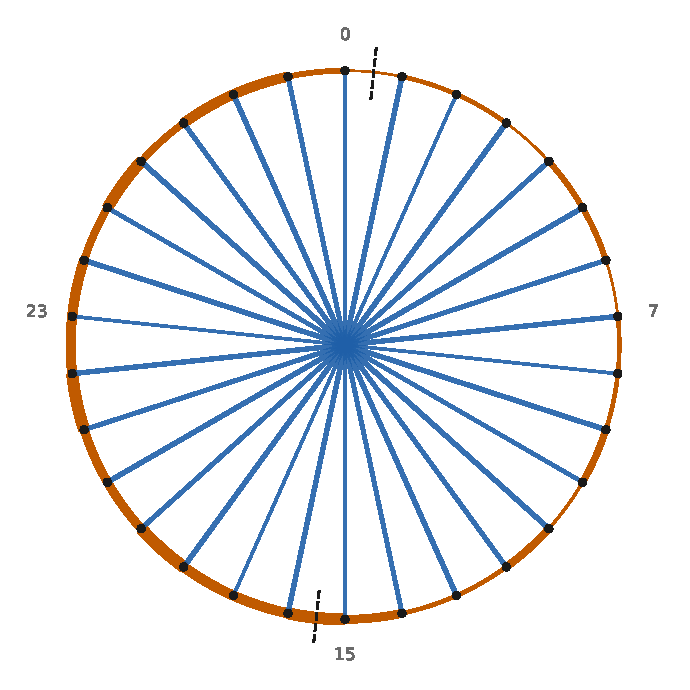
\includegraphics[width=0.46\textwidth]{fig_ring.pdf}
\caption{The instance $\mathcal{R}(u,v)$ for Table~\ref{tab:seq}: 30 nodes, with node~0 at the top and indices increasing clockwise. Blue chords are the 15 crossing demands, with width proportional to size. The width of each orange ring edge is proportional to the filler amount $\varphi_e$ on that edge. The dashed marks show the cut $\{0,15\}$ used in Lemma~\ref{lem:lstar}.}\label{fig:ring}
\end{figure}

\begin{lemma}[load identity]\label{lem:load}
Fix an unsplittable routing of the crossing demands. Put $z_i=v_i$ if demand $i$ is routed clockwise and $z_i=-u_i$ otherwise. If every filler is routed along its own edge, then for $k=1,\dots,m$ the load of edge $k-1$ is $\bar B+\Delta_k(z)$ and the load of edge $m+k-1$ is $\bar B-\Delta_k(z)$.
\end{lemma}

\begin{proof}
Edge $k-1$ lies on the clockwise path of crossing demand $i$ exactly when $i\le k$. Edge $m+k-1$ lies on it exactly when $i>k$.
Compare with~$\sigma$. Routing demand $i$ clockwise adds $v_i$ to each edge of its clockwise path and removes $v_i$ from each edge of its counterclockwise path. Routing it counterclockwise removes $u_i$ from the clockwise edges and adds $u_i$ to the counterclockwise ones.
Summing over~$i$, the load of edge $k-1$ changes by $\Delta_k(z)$ relative to~$\sigma$, and the load of edge $m+k-1$ changes by $-\Delta_k(z)$.
Under $\sigma$, with the fillers on their own edges, every edge carries $B_e+\varphi_e=\bar B$.
\end{proof}

So among unsplittable routings that keep every filler on its own edge, the best maximum load is $\bar B+\alpha_{\{1,\dots,m\}}(u,v)$.
The difficulty is that a filler may instead be routed the long way round, which can lower the maximum load (see Proposition~\ref{prop:ae}).

\begin{lemma}\label{lem:lstar}
$L^*(\mathcal{R}(u,v))=\bar B$.
\end{lemma}

\begin{proof}
The routing $\sigma$, together with every filler on its own edge, is a split routing in which every edge carries load~$\bar B$. Hence $L^*\le\bar B$.
For the matching lower bound, fix any edge $e$ and its opposite edge $e+m$.
Each crossing demand contributes $u_i$ to one of $B_e,B_{e+m}$ and $v_i$ to the other. Hence $B_e+B_{e+m}=\sum_i(u_i+v_i)$, and therefore $\varphi_e+\varphi_{e+m}=2\bar B-\sum_i(u_i+v_i)$.
Deleting edges $e$ and $e+m$ splits the cycle into two paths of $m$ nodes each. Every crossing demand, and every filler on $e$ or $e+m$, has one endpoint on each path. These separated demands have total size $\sum_i(u_i+v_i)+\varphi_e+\varphi_{e+m}=2\bar B$.
Any split routing must send all of this flow through $e$ or $e+m$. So $\mathrm{load}(e)+\mathrm{load}(e+m)\ge 2\bar B$, and the maximum load is at least~$\bar B$.
\end{proof}

\begin{lemma}[fillers]\label{lem:filler}
Fix the routing of the crossing demands, and let $\ell_e$ be the resulting load of edge $e$ when every filler is on its own edge.
Suppose the fillers on edge $e$ that are routed the long way have total size $r_e$, and let $R=\sum_er_e$. Then the load of edge $e$ is $\ell_e+R-2r_e$.
Let $\ell_{(1)}\ge\ell_{(2)}$ be the two largest entries of the vector $(\ell_e)_e$, counted with multiplicity. If some choice of the $r_e$ gives maximum load at most~$T$, then
(i)~$\ell_{(1)}\le T$, or
(ii)~$\ell_{(2)}\le T$ and $\ell_{(1)}+\ell_{(2)}\le 2T$.
(The proof gives $\ell_{(2)}<T$ in~(ii); we state the weaker form, which is the one the code tests.)
\end{lemma}

\begin{proof}
A filler on edge $e$ that goes the long way leaves edge~$e$ and loads every other edge. This gives the load formula.
Suppose that $\ell_{(1)}=\ell_{e_1}>T$, and let $e_2\neq e_1$ be an edge with $\ell_{e_2}=\ell_{(2)}$.
From $\ell_{e_1}+R-2r_{e_1}\le T<\ell_{e_1}$ we get $2r_{e_1}>R$. Since $r_{e_2}\le R-r_{e_1}$, the load of~$e_2$ is
\[
\ell_{e_2}+R-2r_{e_2}\ \ge\ \ell_{e_2}+2r_{e_1}-R\ >\ \ell_{e_2},
\]
so $\ell_{(2)}<T$.
Adding the loads of $e_1$ and $e_2$ gives $\ell_{e_1}+\ell_{e_2}+2(R-r_{e_1}-r_{e_2})\ge\ell_{(1)}+\ell_{(2)}$, and the left side is at most $2T$.
\end{proof}

\begin{theorem}\label{thm:ring}
Let $\mathcal{R}=\mathcal{R}(u,v)$ for the sequence of Table~\ref{tab:seq}. It has $30$ nodes, $55$ demands and $D=1$, and $L^*=15/2$ and $L=69/8$. Hence $L=L^*+\tfrac98D$ and $\rho\ge 9/8$.
\end{theorem}

\begin{proof}
By Lemma~\ref{lem:lstar}, $L^*=\bar B=15/2$.

\emph{$L\le 69/8$.} Route crossing demands $3,4,6,8,11,13$ clockwise and the others counterclockwise, which is the sign vector of Table~\ref{tab:seq}. Keep every filler on its own edge. By Lemma~\ref{lem:load} the maximum load is $15/2+9/8$.

\emph{$L\ge 69/8$.} All demands are multiples of $1/16$, so all loads are too. Suppose some unsplittable routing had maximum load below $69/8$. Its maximum load would then be at most $T:=137/16$.
Fix any of the $2^{15}$ routings of the crossing demands and let $\ell$ be as in Lemma~\ref{lem:filler}.
By Lemma~\ref{lem:load} and Theorem~\ref{thm:seq}, $\ell_{(1)}=15/2+\max_{1\le k\le 15}|\Delta_k(z)|\ge 69/8>T$, so case~(i) never applies.
Case~(ii) holds for only $8$ of the $32768$ routings.
For each of these 8, we decide exactly, by dynamic programming, whether a filler rerouting reaches maximum load at most~$T$.
Let $\Sigma_e$ be the set of subset sums of the filler pieces on edge~$e$. For each $R\in\{0,\tfrac1{16},\dots,\sum_e\varphi_e\}$, where $\sum_e\varphi_e=225/8$, the DP asks whether there are $r_e\in\Sigma_e$ with $\sum_er_e=R$ and $2r_e\ge\ell_e+R-T$ for every~$e$. This is a subset-sum recursion over the 30 edges.
No routing passes. Two separately written implementations of this argument agree: \texttt{ring\_exact.py}, which uses numba, and \texttt{certificate.py}, which is pure Python with big-integer bitsets. Each finishes in seconds.
\end{proof}

A third program, \texttt{check\_minsum.py}, checks the bound without Lemma~\ref{lem:filler}. It was written separately by a reviewing agent.
For every crossing routing and every~$R$, it computes the smallest admissible $r_e\in\Sigma_e$ (with $r_e\le R$ and $2r_e\ge\ell_e+R-T$) for each edge. Their sum already exceeds~$R$ in every case. The program takes a few minutes.

\paragraph{One demand per node pair.}
In $\mathcal{R}(u,v)$, some node pairs carry two filler pieces. If an instance must have at most one demand per node pair, we subdivide edges.

\begin{lemma}[subdivision]\label{lem:sub}
Let $I$ be a ring loading instance, let $e=\{a,a+1\}$ be an edge, and let $q$ be a demand of size~$d$ between $a$ and $a+1$.
Insert a new node $x$ that splits $e$ into $e'=\{a,x\}$ and $e''=\{x,a+1\}$, and replace $q$ by a demand of size $d$ between $a$ and~$x$. Call the result~$I'$. Then:
\begin{enumerate}[label=(\alph*),leftmargin=*]
\item $L(I')\ge L(I)$ and $L^*(I')\ge L^*(I)$;
\item every split or unsplittable routing of $I$ in which $q$ is routed entirely through~$e$ gives a routing of $I'$ with the same maximum load.
\end{enumerate}
\end{lemma}

\begin{proof}
(a)~Take any routing of~$I'$, and route each demand of~$I$ in the same direction or directions, with the same fractions.
A demand other than~$q$ uses $e'$ in $I'$ exactly when it uses $e''$, and exactly when it uses $e$ in~$I$. The demand~$q$, routed the short way, uses $e'$ in $I'$ and $e$ in~$I$. Routed the long way, it uses neither, but it uses every other edge in both instances.
So the load of $e$ in $I$ equals the load of $e'$ in~$I'$, and every other edge of $I$ has the same load in both instances. Hence the maximum load in $I'$ is at least that in~$I$.
(b)~Keep all directions. Every edge of $I$, with $e$ replaced by~$e'$, keeps its load, and $e''$ carries the load of $e$ minus~$d$.
\end{proof}

\begin{corollary}\label{cor:distinct}
Apply Lemma~\ref{lem:sub} to $\mathcal{R}(u,v)$ of Theorem~\ref{thm:ring} once on each of the 13 edges that carry two filler pieces, moving the smaller piece. The result has $43$ nodes and $55$ demands on $55$ distinct node pairs, with $D=1$, $L^*=15/2$ and $L=69/8$.
\end{corollary}

\begin{proof}
Lemma~\ref{lem:sub}(a), applied 13 times, gives $L^*\ge15/2$ and $L\ge69/8$.
Both the split routing $\sigma$ of Lemma~\ref{lem:lstar} and the unsplittable routing used in the proof of Theorem~\ref{thm:ring} keep every filler on its own edge. So Lemma~\ref{lem:sub}(b) gives $L^*\le15/2$ and $L\le69/8$.
\texttt{certificate.py} builds this instance, checks that the node pairs are distinct and that both routings keep their maximum loads, and writes it to the repository.
\end{proof}

\begin{proposition}\label{prop:ae}
\begin{enumerate}[label=(\alph*),leftmargin=*]
\item Let $(u',v')$ be AlphaEvolve's published sequence for Problem~6.61 \cite{AERepo}, with every entry read as the exact binary rational it represents. Then $\alpha_K(u',v')=1.1190475\ldots$ for $K=\{1,\dots,14\}$ and for $K=\{0,\dots,15\}$, while the lift $\mathcal{R}(u',v')$ satisfies $L-L^*\le 1.0823\,D$.
\item Let $(u'',v'')$ be the polished sequence with denominator~$84$ and $\alpha_K(u'',v'')=47/42$. Its lift $\mathcal{R}(u'',v'')$ has $D=1$, $L^*=53/7$ and $L=26/3$, so $L-L^*=\tfrac{23}{21}D$.
\end{enumerate}
In both cases the gap is below $\tfrac{11}{10}D$.
\end{proposition}

\begin{proof}
In both cases $L^*$ is the value $\bar B$ given by Lemma~\ref{lem:lstar}, computed exactly.
For~(a), a mixed-integer solver supplies an unsplittable routing. We evaluate that routing again in exact rational arithmetic, so the bound does not depend on solver tolerances.
For~(b), the bound $L\ge 26/3$ is proved as in Theorem~\ref{thm:ring}: $23$ of the $2^{15}$ crossing routings pass the test of Lemma~\ref{lem:filler}, and the DP rules out every one of them.
The bound $L\le26/3$ comes from an explicit routing that sends filler pieces of total size $13/42$ the long way. Its exact maximum load is $26/3$.
\end{proof}

In~(b), keeping every filler on its own edge would leave a gap of at least $47/42$ (Lemma~\ref{lem:load}), and rerouting fillers lowers it to $23/21=46/42$.
So the sequence bound of~\cite{GGTW25} does not transfer to $\rho$ through this construction.
The sequence of Table~\ref{tab:seq} does transfer without loss, although, as Remark~\ref{rem:others} shows, not every $9/8$ sequence does.
The construction of \cite[Lemma~7]{Dau22} does lift it: rozetyp computed a ring gap of exactly $\tfrac{47}{42}D$ from the exact certificate of \cite{Yad26} \cite{Roz26}.

\section{How the instance was found}\label{sec:search}

The sequence was found by computer search over $(u,v)$ that maximises $\alpha_{\{1,\dots,m-1\}}(u,v)$.
\begin{itemize}[leftmargin=*]
\item \emph{Exact evaluator.} A depth-first branch and bound over~$z$. The condition $\max_k|\Delta_k(z)|\le\alpha$ says that all prefix sums of $z$ lie in an interval of length~$\alpha$. A partial sign vector can therefore be pruned as soon as the range of its prefix sums reaches the best value found so far. The evaluator agreed with brute force on 200 random instances.
\item \emph{Local ascent.} For a fixed~$z$, each $\Delta_k(z)$ is linear in $(u,v)$, so $\alpha$ is a min--max of linear pieces. At the current point we collect the sign vectors within a small tolerance of the minimum. For each, we keep the piece that attains its maximum. We then solve a linear program for the step, inside a trust region, that most increases the smallest of these pieces, followed by a line search.
\item \emph{Iterated local search.} Perturbations, insertion and deletion of terms, splitting a term in two, and reversal, combined with the ascent step. Acceptance is annealed, and the search restarts from the best point found so far after $25$ steps without improvement.
\end{itemize}
Chains started at random points stalled at $11/10$. Chains started at AlphaEvolve's sequence stalled at $47/42$. With restarts from the elite point, four chains reached $9/8$ independently, the fastest after $37$ seconds on one CPU core. We rationalised the result to denominator~$16$ and verified it exactly.

\paragraph{A remark on the excluded region.}
The scoring function published with \cite{AERepo}, in notebook \texttt{experiments/ring\_loading\_problem}, returns $-1$ for sequences with $m>18$. It also returns $-1$ for sequences with $\min_iu_i<0.05$ or $\min_iv_i<0.05$.
All three of our sequences with value $9/8$ contain an entry equal to~$0$, so they lie in the region that this scoring function excludes.
We do not know whether this filter was active in the runs reported in \cite{GGTW25}. We mention it only because it may explain why the search there stopped at $47/42$.

\paragraph{Search beyond $9/8$.}
We ran about $1.5\times10^5$ further iterations of the local search for $15\le m\le 28$, including chains seeded at the $9/8$ sequences.
We also ran a search that maximised $\alpha_{\{1,\dots,m\}}$, the objective that Lemma~\ref{lem:load} ties to the ring: six chains for three hours.
Every run stalled at exactly $9/8$.
An exact mixed-integer program for a local ascent step around each $9/8$ sequence found no improving direction.
This is evidence only that $9/8$ is a barrier for this kind of local search. It is not evidence about $\beta$ or~$\rho$.

\section{Open questions}

The known ranges are now $9/8\le\rho\le13/10$ and $9/8\le\beta\le19/14$.
Is $\rho=9/8$, or $\beta=9/8$?
A first step would be a structural explanation of the $9/8$ instances. In Table~\ref{tab:seq}, seven rows have $u_k+v_k=1$, and several rows repeat: rows 1, 7 and 13; rows 2 and 8; rows 3 and 9; rows 6 and 14. There are also two zeros. These features might generalise to a family.
Our filler choice does not always lift a sequence without loss (Proposition~\ref{prop:ae}), but the construction of \cite[Lemma~7]{Dau22} does \cite{Mak26,Roz26}.

\section*{Code and data}
The instances (exact rational data), the two verifiers and the search code are available at \url{https://github.com/Thanh-Van-2001/ring-loading-9-8}.
\texttt{python certificate.py} reproduces the exact numbers of Sections~\ref{sec:seq} and~\ref{sec:ring} in about two seconds, including Table~\ref{tab:seq}, Corollary~\ref{cor:distinct} and Proposition~\ref{prop:ae}(b).
\texttt{ae\_raw\_lift.py} reproduces Proposition~\ref{prop:ae}(a), and \texttt{check\_minsum.py} gives the third check of Theorem~\ref{thm:ring}.

\section*{Use of AI tools}
The search code, the verification programs and a first draft of this note were written with Claude (Anthropic) in Claude Code, at the author's direction.
The author takes responsibility for the content.
Every mathematical claim rests on exact computations that the reader can rerun with the code above.

\begin{thebibliography}{99}\small

\bibitem{AS26}
D.~Alemán Espinosa and N.~Schlomberg.
\newblock Pinning on tight cuts: improved algorithm and bounds for unsplittable multicommodity flows in outerplanar graphs.
\newblock In \emph{Proc.\ 53rd International Colloquium on Automata, Languages, and Programming (ICALP)}, 2026. arXiv:2606.04456.

\bibitem{AERepo}
Google DeepMind.
\newblock AlphaEvolve repository of problems, Problem~61 (ring loading; Problem~6.61 in \cite{GGTW25}) and notebook \texttt{experiments/ring\_loading\_problem}.
\newblock \url{https://github.com/google-deepmind/alphaevolve_repository_of_problems}, accessed 24 November 2026.

\bibitem{CS94}
S.~Cosares and I.~Saniee.
\newblock An optimization problem related to balancing loads on {SONET} rings.
\newblock \emph{Telecommunication Systems}, 3:165--181, 1994. doi:10.1007/BF02110141.

\bibitem{Dau22}
K.~Däubel.
\newblock An improved upper bound for the ring loading problem.
\newblock \emph{SIAM Journal on Discrete Mathematics}, 36(2):867--887, 2022. doi:10.1137/20M1319395. arXiv:1904.02119.

\bibitem{Mak26}
Maks23 (GitHub user), with comments by V.~Yadav, K.~Däubel, C.~Toledo and rozetyp.
\newblock Problem 61 (Ring Loading): new lower bound $C\ge9/8$, exact certificate with $m=14$.
\newblock Issue~\#12 of \cite{AERepo}, 8 October 2026. \url{https://github.com/google-deepmind/alphaevolve_repository_of_problems/issues/12}.

\bibitem{Roz26}
rozetyp (GitHub user).
\newblock Ring loading instances built from the $47/42$ and $9/8$ certificates, solved exactly with CP-SAT.
\newblock \url{https://github.com/rozetyp/ring-loading-47-42}, 23 November 2026.

\bibitem{Yad26}
V.~Yadav.
\newblock Problem 61 (ring loading): exact rational instance with $\alpha=47/42$.
\newblock Issue~\#11 of \cite{AERepo}, 6 October 2026. \url{https://github.com/google-deepmind/alphaevolve_repository_of_problems/issues/11}.

\bibitem{GGTW25}
B.~Georgiev, J.~Gómez-Serrano, T.~Tao, and A.~Z.~Wagner.
\newblock Mathematical exploration and discovery at scale.
\newblock arXiv:2511.02864, 2025.

\bibitem{SSW98}
A.~Schrijver, P.~Seymour, and P.~Winkler.
\newblock The ring loading problem.
\newblock \emph{SIAM Journal on Discrete Mathematics}, 11(1):1--14, 1998. doi:10.1137/S0895480195294994.

\bibitem{Sku16}
M.~Skutella.
\newblock A note on the ring loading problem.
\newblock \emph{SIAM Journal on Discrete Mathematics}, 30(1):327--342, 2016. doi:10.1137/14099588X.

\end{thebibliography}
\end{document}
